% Options for packages loaded elsewhere
\PassOptionsToPackage{unicode}{hyperref}
\PassOptionsToPackage{hyphens}{url}
\PassOptionsToPackage{dvipsnames,svgnames,x11names}{xcolor}
%
\documentclass[
  11pt,
]{article}

\usepackage{amsmath,amssymb}
\usepackage{setspace}
\usepackage{iftex}
\ifPDFTeX
  \usepackage[T1]{fontenc}
  \usepackage[utf8]{inputenc}
  \usepackage{textcomp} % provide euro and other symbols
\else % if luatex or xetex
  \usepackage{unicode-math}
  \defaultfontfeatures{Scale=MatchLowercase}
  \defaultfontfeatures[\rmfamily]{Ligatures=TeX,Scale=1}
\fi
\usepackage{lmodern}
\ifPDFTeX\else  
    % xetex/luatex font selection
\fi
% Use upquote if available, for straight quotes in verbatim environments
\IfFileExists{upquote.sty}{\usepackage{upquote}}{}
\IfFileExists{microtype.sty}{% use microtype if available
  \usepackage[]{microtype}
  \UseMicrotypeSet[protrusion]{basicmath} % disable protrusion for tt fonts
}{}
\makeatletter
\@ifundefined{KOMAClassName}{% if non-KOMA class
  \IfFileExists{parskip.sty}{%
    \usepackage{parskip}
  }{% else
    \setlength{\parindent}{0pt}
    \setlength{\parskip}{6pt plus 2pt minus 1pt}}
}{% if KOMA class
  \KOMAoptions{parskip=half}}
\makeatother
\usepackage{xcolor}
\usepackage[margin=1in]{geometry}
\setlength{\emergencystretch}{3em} % prevent overfull lines
\setcounter{secnumdepth}{5}
% Make \paragraph and \subparagraph free-standing
\ifx\paragraph\undefined\else
  \let\oldparagraph\paragraph
  \renewcommand{\paragraph}[1]{\oldparagraph{#1}\mbox{}}
\fi
\ifx\subparagraph\undefined\else
  \let\oldsubparagraph\subparagraph
  \renewcommand{\subparagraph}[1]{\oldsubparagraph{#1}\mbox{}}
\fi

\usepackage{color}
\usepackage{fancyvrb}
\newcommand{\VerbBar}{|}
\newcommand{\VERB}{\Verb[commandchars=\\\{\}]}
\DefineVerbatimEnvironment{Highlighting}{Verbatim}{commandchars=\\\{\}}
% Add ',fontsize=\small' for more characters per line
\usepackage{framed}
\definecolor{shadecolor}{RGB}{241,243,245}
\newenvironment{Shaded}{\begin{snugshade}}{\end{snugshade}}
\newcommand{\AlertTok}[1]{\textcolor[rgb]{0.68,0.00,0.00}{#1}}
\newcommand{\AnnotationTok}[1]{\textcolor[rgb]{0.37,0.37,0.37}{#1}}
\newcommand{\AttributeTok}[1]{\textcolor[rgb]{0.40,0.45,0.13}{#1}}
\newcommand{\BaseNTok}[1]{\textcolor[rgb]{0.68,0.00,0.00}{#1}}
\newcommand{\BuiltInTok}[1]{\textcolor[rgb]{0.00,0.23,0.31}{#1}}
\newcommand{\CharTok}[1]{\textcolor[rgb]{0.13,0.47,0.30}{#1}}
\newcommand{\CommentTok}[1]{\textcolor[rgb]{0.37,0.37,0.37}{#1}}
\newcommand{\CommentVarTok}[1]{\textcolor[rgb]{0.37,0.37,0.37}{\textit{#1}}}
\newcommand{\ConstantTok}[1]{\textcolor[rgb]{0.56,0.35,0.01}{#1}}
\newcommand{\ControlFlowTok}[1]{\textcolor[rgb]{0.00,0.23,0.31}{#1}}
\newcommand{\DataTypeTok}[1]{\textcolor[rgb]{0.68,0.00,0.00}{#1}}
\newcommand{\DecValTok}[1]{\textcolor[rgb]{0.68,0.00,0.00}{#1}}
\newcommand{\DocumentationTok}[1]{\textcolor[rgb]{0.37,0.37,0.37}{\textit{#1}}}
\newcommand{\ErrorTok}[1]{\textcolor[rgb]{0.68,0.00,0.00}{#1}}
\newcommand{\ExtensionTok}[1]{\textcolor[rgb]{0.00,0.23,0.31}{#1}}
\newcommand{\FloatTok}[1]{\textcolor[rgb]{0.68,0.00,0.00}{#1}}
\newcommand{\FunctionTok}[1]{\textcolor[rgb]{0.28,0.35,0.67}{#1}}
\newcommand{\ImportTok}[1]{\textcolor[rgb]{0.00,0.46,0.62}{#1}}
\newcommand{\InformationTok}[1]{\textcolor[rgb]{0.37,0.37,0.37}{#1}}
\newcommand{\KeywordTok}[1]{\textcolor[rgb]{0.00,0.23,0.31}{#1}}
\newcommand{\NormalTok}[1]{\textcolor[rgb]{0.00,0.23,0.31}{#1}}
\newcommand{\OperatorTok}[1]{\textcolor[rgb]{0.37,0.37,0.37}{#1}}
\newcommand{\OtherTok}[1]{\textcolor[rgb]{0.00,0.23,0.31}{#1}}
\newcommand{\PreprocessorTok}[1]{\textcolor[rgb]{0.68,0.00,0.00}{#1}}
\newcommand{\RegionMarkerTok}[1]{\textcolor[rgb]{0.00,0.23,0.31}{#1}}
\newcommand{\SpecialCharTok}[1]{\textcolor[rgb]{0.37,0.37,0.37}{#1}}
\newcommand{\SpecialStringTok}[1]{\textcolor[rgb]{0.13,0.47,0.30}{#1}}
\newcommand{\StringTok}[1]{\textcolor[rgb]{0.13,0.47,0.30}{#1}}
\newcommand{\VariableTok}[1]{\textcolor[rgb]{0.07,0.07,0.07}{#1}}
\newcommand{\VerbatimStringTok}[1]{\textcolor[rgb]{0.13,0.47,0.30}{#1}}
\newcommand{\WarningTok}[1]{\textcolor[rgb]{0.37,0.37,0.37}{\textit{#1}}}

\providecommand{\tightlist}{%
  \setlength{\itemsep}{0pt}\setlength{\parskip}{0pt}}\usepackage{longtable,booktabs,array}
\usepackage{calc} % for calculating minipage widths
% Correct order of tables after \paragraph or \subparagraph
\usepackage{etoolbox}
\makeatletter
\patchcmd\longtable{\par}{\if@noskipsec\mbox{}\fi\par}{}{}
\makeatother
% Allow footnotes in longtable head/foot
\IfFileExists{footnotehyper.sty}{\usepackage{footnotehyper}}{\usepackage{footnote}}
\makesavenoteenv{longtable}
\usepackage{graphicx}
\makeatletter
\def\maxwidth{\ifdim\Gin@nat@width>\linewidth\linewidth\else\Gin@nat@width\fi}
\def\maxheight{\ifdim\Gin@nat@height>\textheight\textheight\else\Gin@nat@height\fi}
\makeatother
% Scale images if necessary, so that they will not overflow the page
% margins by default, and it is still possible to overwrite the defaults
% using explicit options in \includegraphics[width, height, ...]{}
\setkeys{Gin}{width=\maxwidth,height=\maxheight,keepaspectratio}
% Set default figure placement to htbp
\makeatletter
\def\fps@figure{htbp}
\makeatother

\usepackage{booktabs}
\usepackage{caption}
\usepackage{longtable}
\usepackage{colortbl}
\usepackage{array}
\makeatletter
\makeatother
\makeatletter
\makeatother
\makeatletter
\@ifpackageloaded{caption}{}{\usepackage{caption}}
\AtBeginDocument{%
\ifdefined\contentsname
  \renewcommand*\contentsname{Table of contents}
\else
  \newcommand\contentsname{Table of contents}
\fi
\ifdefined\listfigurename
  \renewcommand*\listfigurename{List of Figures}
\else
  \newcommand\listfigurename{List of Figures}
\fi
\ifdefined\listtablename
  \renewcommand*\listtablename{List of Tables}
\else
  \newcommand\listtablename{List of Tables}
\fi
\ifdefined\figurename
  \renewcommand*\figurename{Figure}
\else
  \newcommand\figurename{Figure}
\fi
\ifdefined\tablename
  \renewcommand*\tablename{Table}
\else
  \newcommand\tablename{Table}
\fi
}
\@ifpackageloaded{float}{}{\usepackage{float}}
\floatstyle{ruled}
\@ifundefined{c@chapter}{\newfloat{codelisting}{h}{lop}}{\newfloat{codelisting}{h}{lop}[chapter]}
\floatname{codelisting}{Listing}
\newcommand*\listoflistings{\listof{codelisting}{List of Listings}}
\makeatother
\makeatletter
\@ifpackageloaded{caption}{}{\usepackage{caption}}
\@ifpackageloaded{subcaption}{}{\usepackage{subcaption}}
\makeatother
\makeatletter
\@ifpackageloaded{tcolorbox}{}{\usepackage[skins,breakable]{tcolorbox}}
\makeatother
\makeatletter
\@ifundefined{shadecolor}{\definecolor{shadecolor}{rgb}{.97, .97, .97}}
\makeatother
\makeatletter
\makeatother
\makeatletter
\makeatother
\ifLuaTeX
  \usepackage{selnolig}  % disable illegal ligatures
\fi
\IfFileExists{bookmark.sty}{\usepackage{bookmark}}{\usepackage{hyperref}}
\IfFileExists{xurl.sty}{\usepackage{xurl}}{} % add URL line breaks if available
\urlstyle{same} % disable monospaced font for URLs
\hypersetup{
  pdftitle={Behind the Curtain: Statistical Insights into Movie Success},
  pdfauthor={Cheng Tang, Mingcan Wang, Yiang Liang, Yuxuan Zhao, Zilu Wang},
  colorlinks=true,
  linkcolor={blue},
  filecolor={Maroon},
  citecolor={Blue},
  urlcolor={Blue},
  pdfcreator={LaTeX via pandoc}}

\title{Behind the Curtain: Statistical Insights into Movie Success}
\author{Cheng Tang, Mingcan Wang, Yiang Liang, Yuxuan Zhao, Zilu Wang}
\date{}

\begin{document}
\maketitle
\ifdefined\Shaded\renewenvironment{Shaded}{\begin{tcolorbox}[frame hidden, interior hidden, borderline west={3pt}{0pt}{shadecolor}, breakable, enhanced, sharp corners, boxrule=0pt]}{\end{tcolorbox}}\fi

\renewcommand*\contentsname{Table of contents}
{
\hypersetup{linkcolor=}
\setcounter{tocdepth}{3}
\tableofcontents
}
\setstretch{1.5}
\hypertarget{introduction}{%
\section{Introduction}\label{introduction}}

In the evolving landscape of cinematic entertainment, the question of
what factors lead a film to be favorably received by audiences has
intrigued producers, directors, and marketers alike. This project,
titled ``Behind the Curtain: Statistical Insights into Movie Success''
embarks on a statistical journey to decipher the complex dynamics
between various film attributes and their resulting viewer ratings,
specifically focusing on the critical threshold of a rating above 7,
often considered a benchmark for success in the industry.

The inception of this analysis is rooted in the premise that a film's
length, budget, viewer engagement (measured through votes), and genre
hold significant sway over its overall reception. Traditionally, the
entertainment industry has relied on anecdotal evidence or isolated case
studies to gauge the potential success of film projects. However, this
project leverages a Generalized Linear Model (GLM) to evaluate these
factors, offering a more empirical basis for understanding cinematic
success.

The data set comprises diverse films spanning various years, genres, and
production scales, enabling a comprehensive analysis that transcends
specific market trends or cultural biases. By employing a generalized
linear regression framework, we aim to predict the likelihood of a film
achieving a rating above 7, transforming subjective notions of quality
and appeal into quantifiable probabilities.

Through this project, the goal is to distill actionable insights that
can guide filmmakers and studios in crafting content that resonates with
viewers. Beyond its immediate application, this study contributes to the
broader discourse on the quantification of artistic and entertainment
value, marking a confluence of creativity and analytics.

\hypertarget{methodology}{%
\section{Methodology}\label{methodology}}

The methodology of the project involves a systematic approach to
understanding the factors contributing to movie success, as measured by
audience ratings. Initially, the data is cleansed and pre-processed,
which includes handling missing values and transforming skewed
distributions through log transformations for variables such as film
length and votes to achieve distributions closer to normal.
Subsequently, a binary variable is created to distinguish films based on
whether they have achieved a rating above 7.

An extensive Exploratory Data Analysis (EDA) is conducted to gain deeper
insights into underlying patterns and relationships. This includes
examining the distributions of key variables, identifying outliers, and
assessing correlations.

The analysis then employs a Generalized Linear Model (GLM), specifically
logistic regression, to examine the influence of various film attributes
on the likelihood of a film receiving a rating above 7, which is
considered indicative of success. The model's predictive power and fit
are assessed through accuracy, sensitivity, specificity, and AUC.

To fine-tune the model, a series of candidate thresholds for
classification are evaluated to identify the optimal balance between
sensitivity and specificity. This involves calculating performance
metrics across different threshold values and selecting the one that
provides the best compromise according to the project's objectives.

The methodology also encompasses evaluation of the model's assumptions
and the fit to the data, ensuring the reliability and validity of the
findings. Finally, based on the insights gained from the EDA and GLM
analysis, strategic recommendations are formulated to guide filmmakers
and producers in aligning their projects with the attributes associated
with higher-rated films.

\hypertarget{exploratory-data-anlaysis}{%
\section{Exploratory Data Anlaysis}\label{exploratory-data-anlaysis}}

\hypertarget{statistical-summary}{%
\subsection{Statistical Summary}\label{statistical-summary}}

\begin{longtable*}{lrrrrrr}
\caption*{
{\large Statistical Summary of Numerical Variables}
} \\ 
\toprule
Variable & Mean & Standard Deviation & Median & Interquartile Range & Minimum & Maximum \\ 
\midrule\addlinespace[2.5pt]
year & 1976.872225 & 23.739365 & 1984.0 & 40.0 & 1894.0 & 2005.0 \\ 
length & 81.745287 & 36.978082 & 90.0 & 26.0 & 1.0 & 399.0 \\ 
budget & 11.948136 & 2.967745 & 12.0 & 3.9 & 2.1 & 23.7 \\ 
votes & 658.969418 & 4370.037987 & 32.0 & 106.0 & 5.0 & 103854.0 \\ 
rating & 5.414328 & 2.069483 & 4.7 & 4.1 & 0.7 & 9.2 \\ 
\bottomrule
\end{longtable*}

\begin{longtable*}{crr}
\caption*{
{\large Frequency and Percentage Summary by Genre}
} \\ 
\toprule
Genre & Frequency & Percentage (\%) \\ 
\midrule\addlinespace[2.5pt]
Action & 698 & 29.24 \\ 
Drama & 684 & 28.66 \\ 
Comedy & 582 & 24.38 \\ 
Animation & 165 & 6.91 \\ 
Documentary & 136 & 5.70 \\ 
Short & 106 & 4.44 \\ 
Romance & 16 & 0.67 \\ 
\bottomrule
\end{longtable*}

\begin{longtable*}{crr}
\caption*{
{\large Frequency and Percentage Summary for Ratings Above 7}
} \\ 
\toprule
Above Rating 7 & Frequency & Percentage (\%) \\ 
\midrule\addlinespace[2.5pt]
0 & 1546 & 64.77 \\ 
1 & 841 & 35.23 \\ 
\bottomrule
\end{longtable*}

\hypertarget{outliers}{%
\subsection{Outliers}\label{outliers}}

\textbf{Proportions of outliers for each numeric variable}

\begin{verbatim}
                          length      budget     votes
Proportion of Outliers 0.1805614 0.004608295 0.1625471
\end{verbatim}

\textbf{Proportions of outliers for numeric variables after log}

\begin{verbatim}
                       length_log  votes_log
Proportion of Outliers  0.1818182 0.03812317
\end{verbatim}

\hypertarget{visualisation}{%
\subsection{Visualisation}\label{visualisation}}

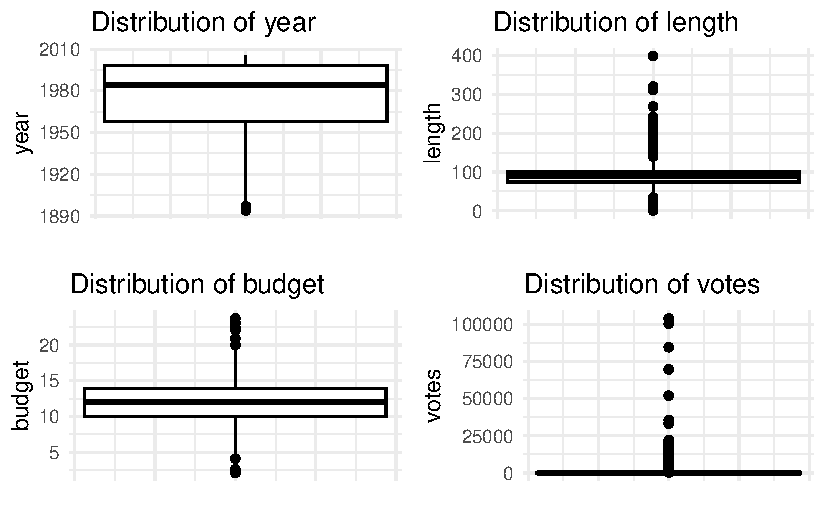
\includegraphics{Group_07_Analysis_files/figure-pdf/unnamed-chunk-12-1.pdf}

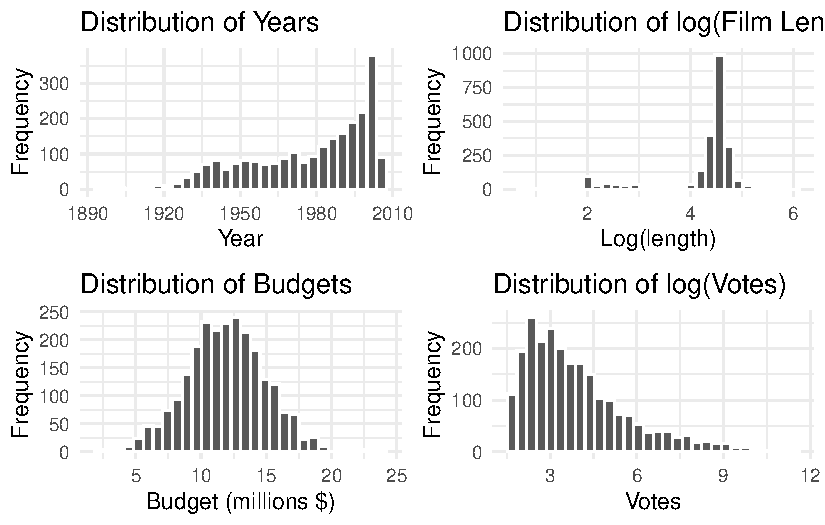
\includegraphics{Group_07_Analysis_files/figure-pdf/unnamed-chunk-13-1.pdf}

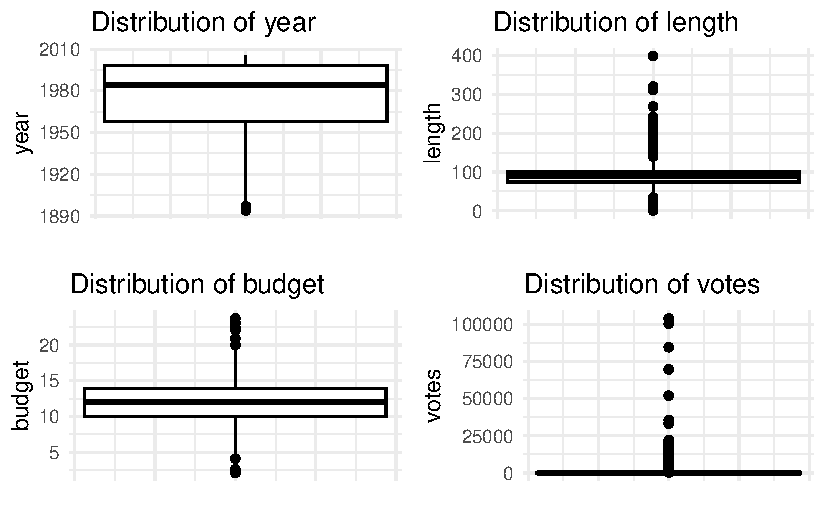
\includegraphics{Group_07_Analysis_files/figure-pdf/unnamed-chunk-14-1.pdf}

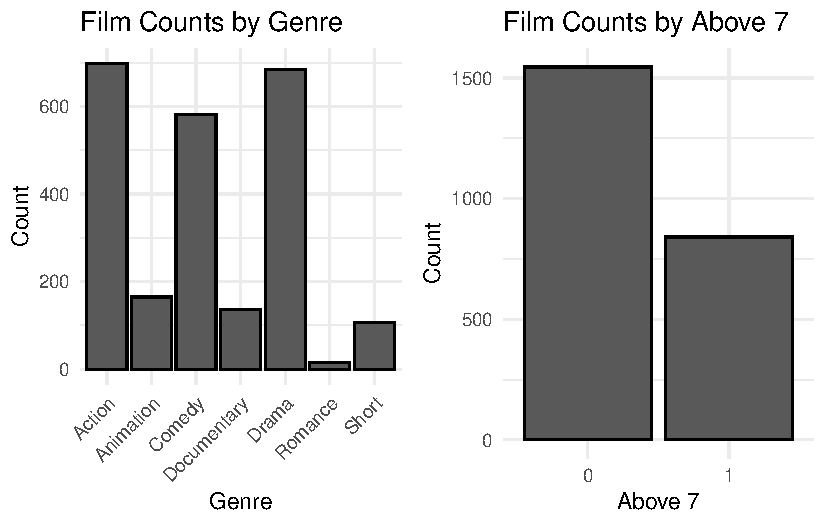
\includegraphics{Group_07_Analysis_files/figure-pdf/unnamed-chunk-15-1.pdf}

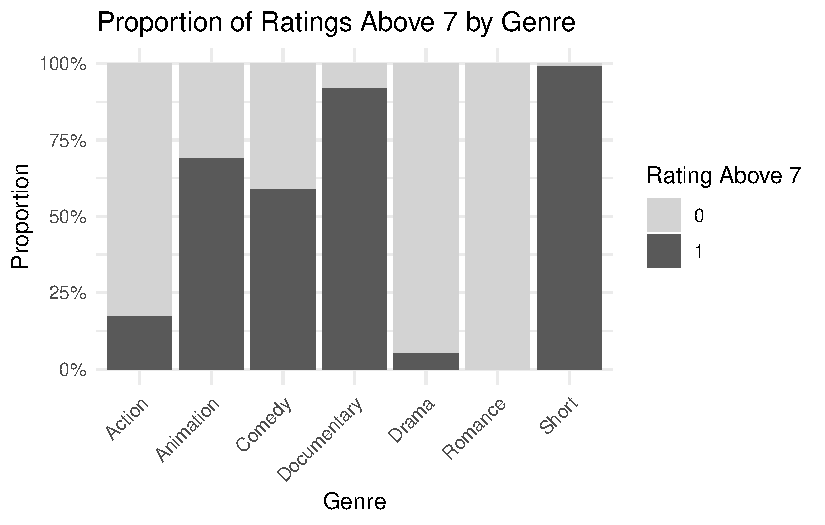
\includegraphics{Group_07_Analysis_files/figure-pdf/unnamed-chunk-16-1.pdf}

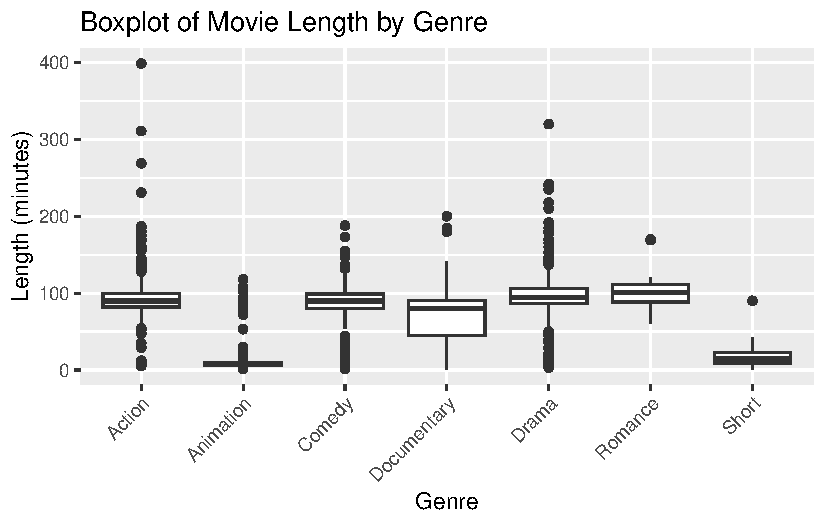
\includegraphics{Group_07_Analysis_files/figure-pdf/unnamed-chunk-17-1.pdf}

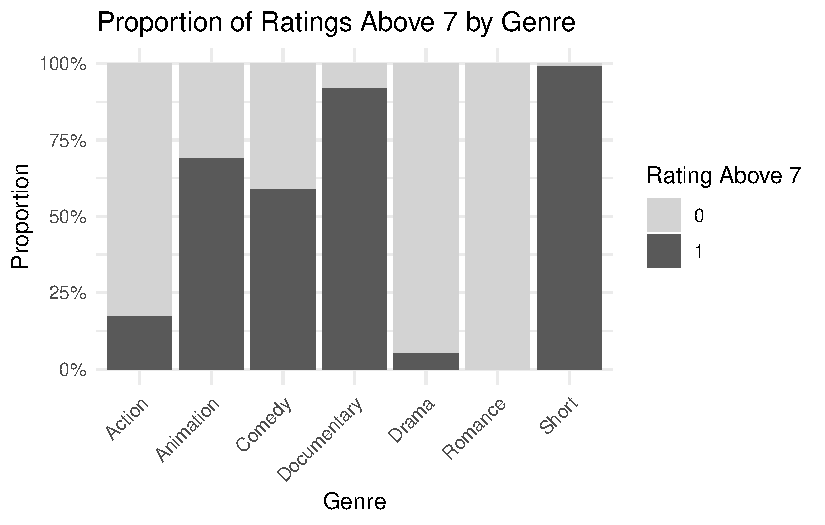
\includegraphics{Group_07_Analysis_files/figure-pdf/unnamed-chunk-18-1.pdf}

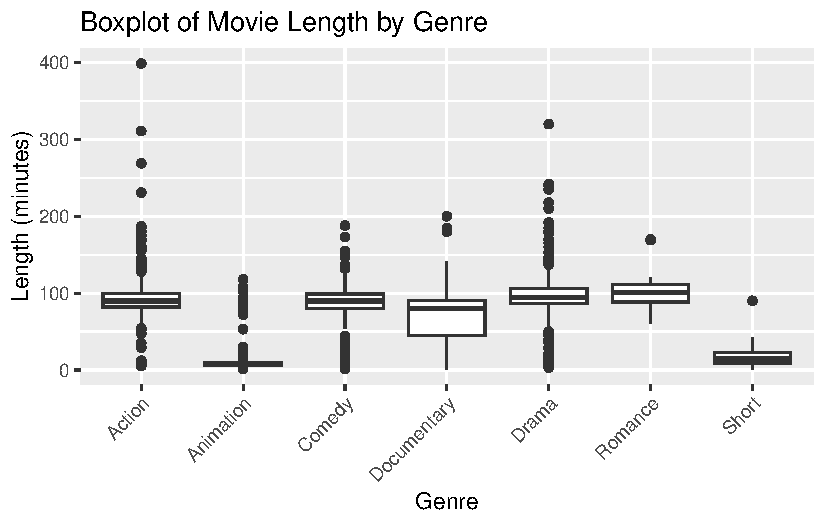
\includegraphics{Group_07_Analysis_files/figure-pdf/unnamed-chunk-19-1.pdf}

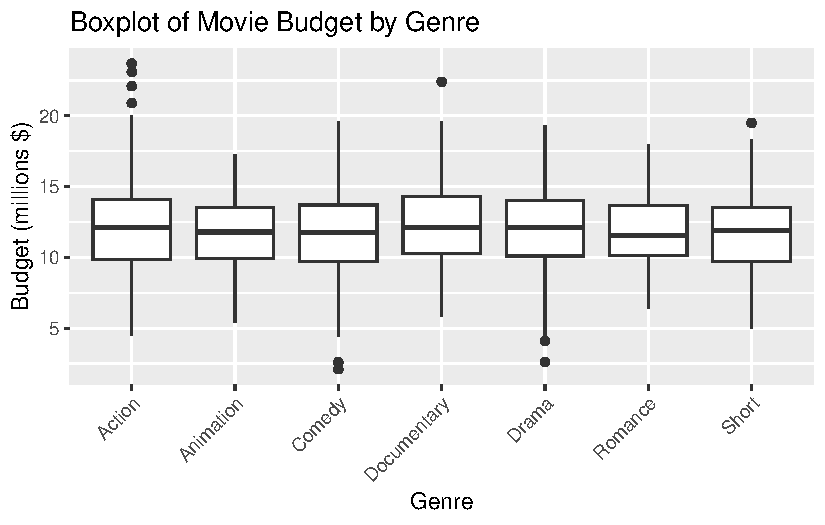
\includegraphics{Group_07_Analysis_files/figure-pdf/unnamed-chunk-19-2.pdf}

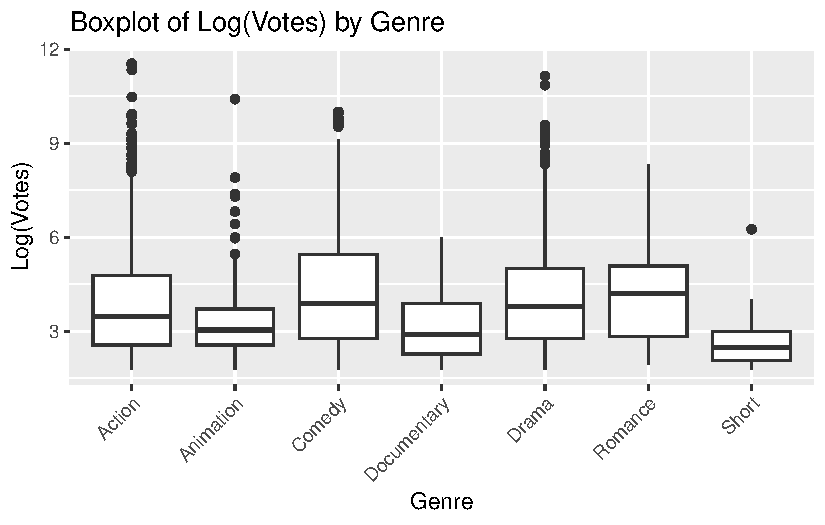
\includegraphics{Group_07_Analysis_files/figure-pdf/unnamed-chunk-19-3.pdf}

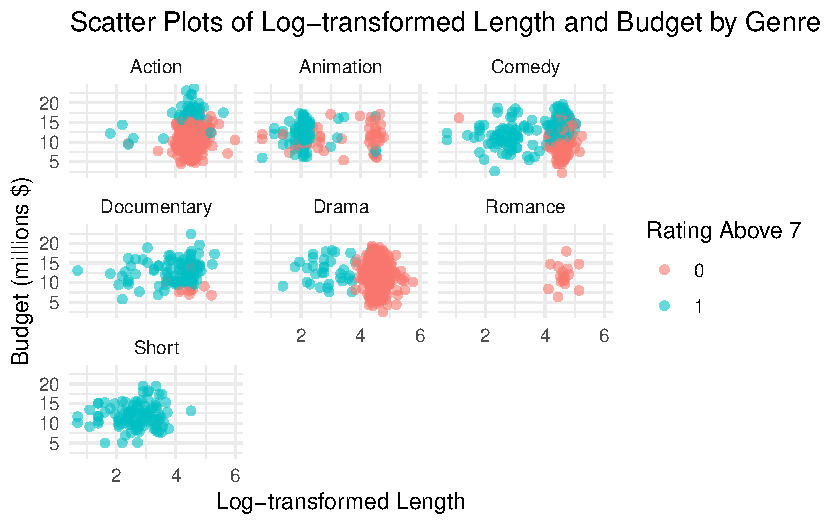
\includegraphics{Group_07_Analysis_files/figure-pdf/unnamed-chunk-20-1.pdf}

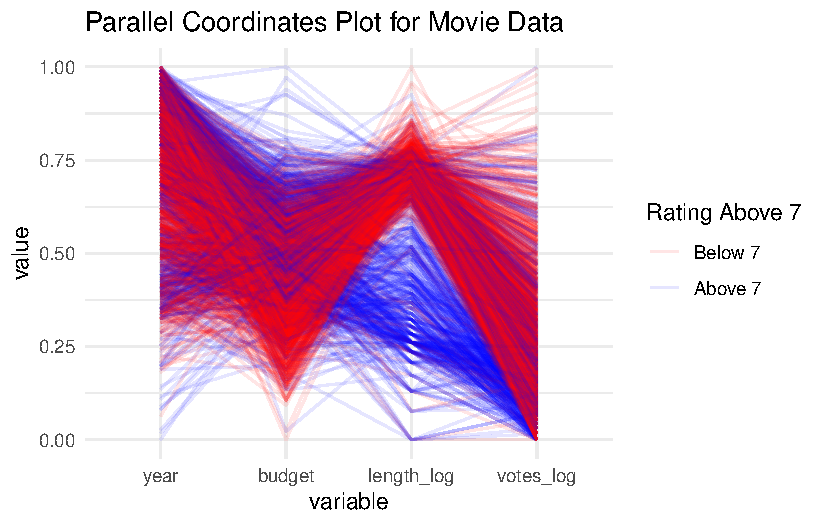
\includegraphics{Group_07_Analysis_files/figure-pdf/unnamed-chunk-21-1.pdf}

\hypertarget{eda-findings}{%
\subsection{EDA Findings}\label{eda-findings}}

In the exploratory data analysis, we observed distinct patterns within
the film data set. The data set predominantly features action (29.24\%),
drama (28.66\%), and comedy (24.38\%) genres, with fewer romantic
(0.67\%) and short films (4.44\%). Notably, only 35\% of movies are
rated above 7.

The length of films is right-skewed, with most under 100 minutes, but
exceptions extending up to 399 minutes. Similarly, the `votes'
distribution is significantly right-skewed, highlighting a disparity in
viewer engagement. After log transformations, the distributions of
`length' and `votes' approached closer to normality but still exhibited
skewness. Conversely, budgets appear nearly normally distributed,
indicating diverse financial investments across films.

There is a medium positive correlation between log-transformed votes and
length, suggesting films of longer duration may engage viewers more. It
is also shown that movies rated above 7 typically have higher budgets.
Genre-wise, short and documentaries stand out with highest proportions
of high-rated films, whereas romance, drama, and action genres show
fewer films surpassing the rating threshold. Short films and animations
are generally shorter, whereas romance tends to be longer. The budget
across various genres does not vary significantly, with action and
documentaries exhibit slightly higher budgets. Lastly, romance genre
films receive the most votes, while short films receive the fewest,
indicating varying audience engagement levels by genre.

\hypertarget{formal-analysis}{%
\section{Formal Analysis}\label{formal-analysis}}

\hypertarget{model-building}{%
\subsection{Model Building}\label{model-building}}

\begin{Shaded}
\begin{Highlighting}[]
\CommentTok{\# Full model}
\NormalTok{glm\_model\_full }\OtherTok{\textless{}{-}} \FunctionTok{glm}\NormalTok{(above\_7 }\SpecialCharTok{\textasciitilde{}}\NormalTok{ year }\SpecialCharTok{+}\NormalTok{ length }\SpecialCharTok{+}\NormalTok{ budget }\SpecialCharTok{+}\NormalTok{ votes }\SpecialCharTok{+}\NormalTok{ genre, }
                      \AttributeTok{family =}\NormalTok{ binomial, }\AttributeTok{data =}\NormalTok{ train\_data)}
\CommentTok{\# Full Model with Log Transformation}
\NormalTok{glm\_model\_log }\OtherTok{\textless{}{-}} \FunctionTok{glm}\NormalTok{(above\_7 }\SpecialCharTok{\textasciitilde{}}\NormalTok{ year }\SpecialCharTok{+}\NormalTok{ length\_log }\SpecialCharTok{+}\NormalTok{ budget }\SpecialCharTok{+}\NormalTok{ votes\_log }\SpecialCharTok{+}\NormalTok{ genre, }
                     \AttributeTok{family =}\NormalTok{ binomial, }\AttributeTok{data =}\NormalTok{ train\_data)}

\CommentTok{\# Model without Year}
\NormalTok{glm\_model\_no\_year }\OtherTok{\textless{}{-}} \FunctionTok{glm}\NormalTok{(above\_7 }\SpecialCharTok{\textasciitilde{}}\NormalTok{ length\_log }\SpecialCharTok{+}\NormalTok{ budget }\SpecialCharTok{+}\NormalTok{ votes\_log }\SpecialCharTok{+}\NormalTok{ genre, }
                        \AttributeTok{family =}\NormalTok{ binomial, }\AttributeTok{data =}\NormalTok{ train\_data)}

\CommentTok{\# Model without Year and Votes\_log}
\NormalTok{glm\_model\_no\_year\_votes }\OtherTok{\textless{}{-}} \FunctionTok{glm}\NormalTok{(above\_7 }\SpecialCharTok{\textasciitilde{}}\NormalTok{ length\_log }\SpecialCharTok{+}\NormalTok{ budget }\SpecialCharTok{+}\NormalTok{ genre, }
                               \AttributeTok{family =}\NormalTok{ binomial, }\AttributeTok{data =}\NormalTok{ train\_data)}
\CommentTok{\# Model without Year and Length\_log}
\NormalTok{glm\_model\_no\_year\_length }\OtherTok{\textless{}{-}} \FunctionTok{glm}\NormalTok{(above\_7 }\SpecialCharTok{\textasciitilde{}}\NormalTok{ votes\_log }\SpecialCharTok{+}\NormalTok{ budget }\SpecialCharTok{+}\NormalTok{ genre, }
                               \AttributeTok{family =}\NormalTok{ binomial, }\AttributeTok{data =}\NormalTok{ train\_data)}
\end{Highlighting}
\end{Shaded}

In this project, the modeling principle involved constructing and
refining a series of logistic regression models to identify key factors
influencing a movie's success, defined as achieving a rating above 7.
The full model included all variables (except film\_id), offering a
comprehensive baseline for analysis.

Subsequent models were developed by applying log transformation and
removing variables based on their statistical significance, assessed
through p-values, and their impact on the model's overall performance.
This iterative process aimed to streamline the model, removing less
impactful variables while observing changes in performance metrics like
accuracy, sensitivity, specificity, and AUC.

\hypertarget{model-selection}{%
\subsection{Model Selection}\label{model-selection}}

\begin{verbatim}
                                             Variables Accuracy Sensitivity
Model 1         year + length + budget + votes + genre   0.8643      0.9179
Model 2 year + length_log + budget + votes_log + genre   0.8755      0.9136
Model 3        length_log + budget + votes_log + genre   0.8755      0.9158
Model 4                    length_log + budget + genre   0.8713      0.9158
Model 5                     votes_log + budget + genre   0.8420      0.9071
        Specificity    AUC       BIC
Model 1      0.7659 0.9372 1007.1164
Model 2      0.8056 0.9405  948.7532
Model 3      0.8016 0.9413  942.5078
Model 4      0.7897 0.9405  941.4027
Model 5      0.7222 0.9009 1192.5274
\end{verbatim}

Model 4 was chosen for further tuning due to its balance between
simplicity and performance. Despite not having the absolute highest
accuracy, it provides high sensitivity (0.9158) and decent specificity
(0.7897), alongside a strong AUC of 0.9405, indicating good
discriminative power. With a BIC of 941.4027, it suggests efficiency in
balancing model fit with complexity. This makes Model 4 a strong
candidate for detailed analysis and threshold optimization.

\hypertarget{model-tuning}{%
\subsection{Model Tuning}\label{model-tuning}}

In fine-tuning our logistic regression model, particularly for an
imbalanced dataset, we focus on optimizing the classification threshold.
This involves systematically assessing various thresholds to find an
optimal balance between Accuracy, Sensitivity, and Specificity. The goal
is to improve model precision by correctly balancing true positive and
negative predictions. This targeted approach ensures our model is better
suited to the specific challenges and objectives of our analysis,
thereby enhancing its predictive reliability and relevance.

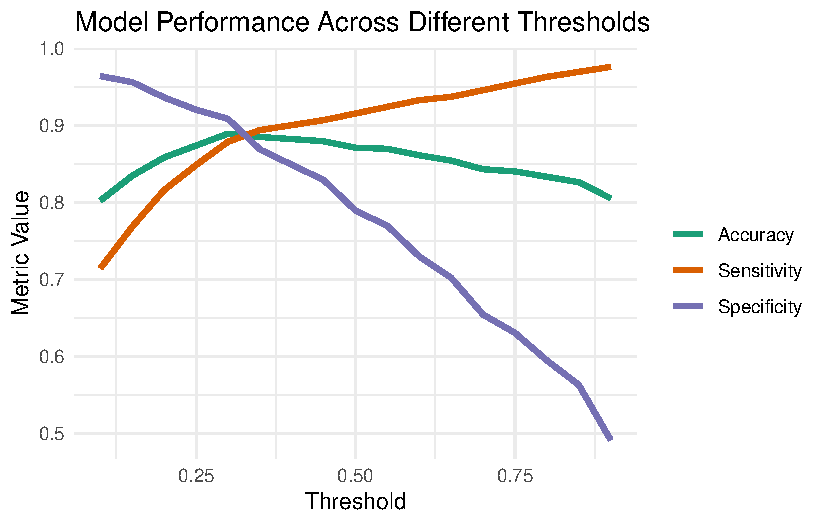
\includegraphics{Group_07_Analysis_files/figure-pdf/unnamed-chunk-26-1.pdf}

\begin{verbatim}
       Metric    Value
1    Accuracy   0.8923
2 Sensitivity   0.8898
3 Specificity   0.8968
4         AUC   0.9405
5         BIC 941.4027
\end{verbatim}

The classification threshold of 0.33, as observed from the plot,
optimally balances accuracy, sensitivity, and specificity. This
threshold reflects a strategic compromise, enhancing the model's ability
to correctly identify films rated above and below 7, without heavily
sacrificing one metric for another.

Model 4, which utilizes length\_log, budget, and genre as predictors,
demonstrates strong predictive performance. With an accuracy of 89.23\%,
it effectively distinguishes between movies rated above and below 7. The
model is equally balanced in terms of sensitivity (88.98\%) and
specificity (89.68\%), indicating it is reliable in identifying both
high-rated and lower-rated films. The AUC value of 0.9405 suggests good
discrimination between the positive and negative classes. Furthermore, a
BIC of 941.4027 reflects the model's efficiency, balancing model
complexity with fit to the data.

\hypertarget{model-interpretation}{%
\subsection{Model Interpretation}\label{model-interpretation}}

\begin{verbatim}

Call:
glm(formula = above_7 ~ length_log + budget + genre, family = binomial, 
    data = train_data)

Coefficients:
                  Estimate Std. Error z value Pr(>|z|)    
(Intercept)        3.66547    1.07287   3.416 0.000634 ***
length_log        -2.79886    0.24870 -11.254  < 2e-16 ***
budget             0.54983    0.03966  13.865  < 2e-16 ***
genreAnimation    -1.61972    0.59253  -2.734 0.006265 ** 
genreComedy        2.66538    0.21699  12.283  < 2e-16 ***
genreDocumentary   4.77889    0.46931  10.183  < 2e-16 ***
genreDrama        -2.54760    0.36048  -7.067 1.58e-12 ***
genreRomance     -13.95741  432.52053  -0.032 0.974257    
genreShort         3.60198    1.08387   3.323 0.000890 ***
---
Signif. codes:  0 '***' 0.001 '**' 0.01 '*' 0.05 '.' 0.1 ' ' 1

(Dispersion parameter for binomial family taken to be 1)

    Null deviance: 2169.73  on 1671  degrees of freedom
Residual deviance:  874.61  on 1663  degrees of freedom
AIC: 892.61

Number of Fisher Scoring iterations: 14
\end{verbatim}

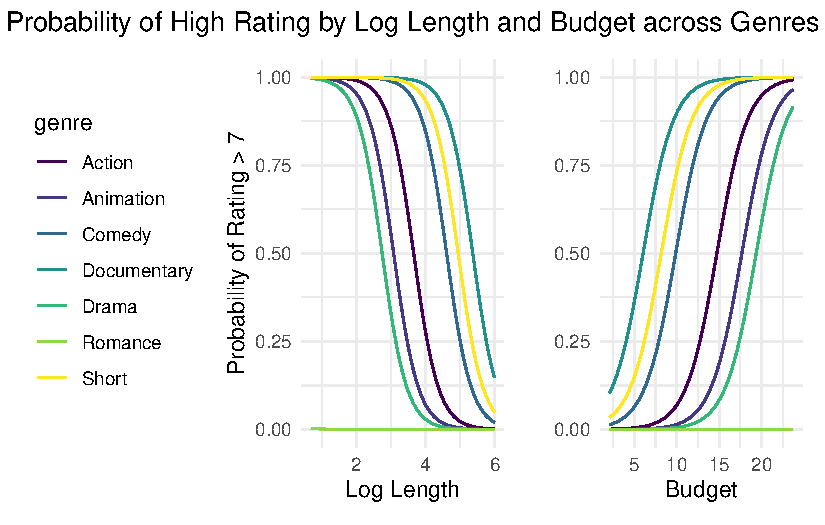
\includegraphics{Group_07_Analysis_files/figure-pdf/unnamed-chunk-29-1.pdf}

\begin{enumerate}
\def\labelenumi{\arabic{enumi}.}
\item
  \textbf{Length of Movies (length\_log)}: There is a significant
  negative relationship between the log-transformed length of movies and
  their likelihood of being rated above 7, with each unit increase
  reducing the odds by 94\% (Odds Ratio = 0.061). This suggests that
  longer movies are less likely to receive high ratings, potentially
  indicating viewer preferences for shorter films or perhaps an
  association with certain film types or genres that are longer but less
  popular.
\item
  \textbf{Budget (budget)}: The budget of a movie shows a significant
  positive association with the likelihood of being rated above 7, with
  each unit increase in budget increasing the odds of a high rating by
  73\% (Odds Ratio = 1.733). This might imply that higher-budget movies,
  which can afford better production quality, actors, and marketing, are
  more likely to be well-received by audiences.
\item
  \textbf{Genre}:

  \begin{itemize}
  \tightlist
  \item
    \textbf{Documentary}: Documentaries have the highest likelihood of
    being rated above 7, 119.188 times more likely than action films.
    This substantial likelihood suggests that documentaries' content
    resonates strongly with audiences, making them the most successful
    genre in this analysis.
  \item
    \textbf{Short and Comedy}: These genres show significant higher
    probability of receiving high ratings compared to action. Short
    films are 36.669 times more likely, and comedies are 14.374 times
    more likely than action films to receive ratings above 7, suggesting
    they are generally well-received or cater to specific audience
    segments that rate them favorably.
  \item
    \textbf{Animation and Drama}: Compared to action, animation and
    drama genres are 80.2\% and 92.2\% less likely, respectively, to be
    rated above 7. This indicates that, despite their popularity, films
    in these genres face greater challenges in surpassing the threshold
    for perceived success, possibly due to differing audience
    expectations or the abundance of content within these categories.
  \item
    \textbf{Romance}: This genre do not show significant effects,
    possibly due to a smaller sample size.
  \end{itemize}
\end{enumerate}

\hypertarget{assumption-checking}{%
\subsection{Assumption Checking}\label{assumption-checking}}

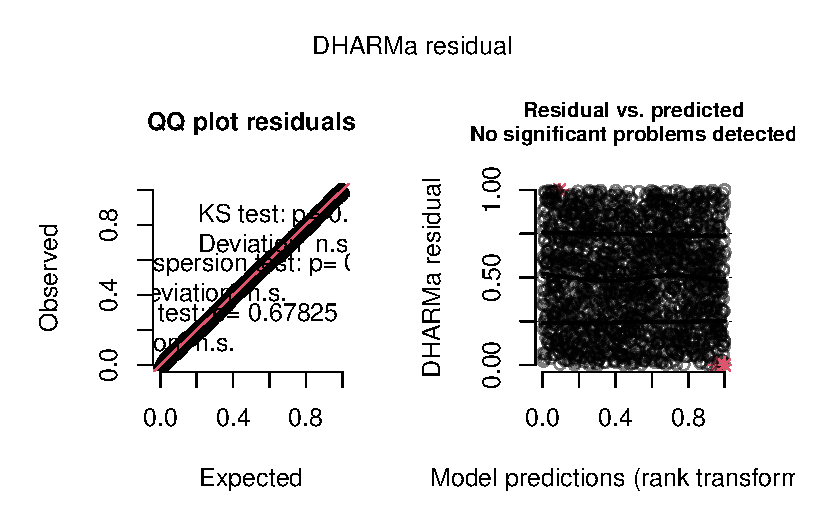
\includegraphics{Group_07_Analysis_files/figure-pdf/unnamed-chunk-35-1.pdf}

The DHARMa diagnostic plots for the generalized linear model indicate
that the model assumptions are largely satisfied. The quantile-quantile
plot reveals that residuals closely follow the expected uniform
distribution, suggesting that the model does not exhibit significant
misfit. The uniformity is further supported by a high p-value in the
Kolmogorov-Smirnov test, indicating no significant deviation from the
expected distribution. The residuals versus predicted values plot shows
no discernible pattern, implying consistent variance across predicted
values and supporting the homoscedasticity assumption. Although there
are a few outliers, they don't appear to systematically affect the
model's validity. Overall, the analysis suggests that the model is
well-fitted to the data under the constraints of GLM assumptions.

\hypertarget{conclusion}{%
\section{Conclusion}\label{conclusion}}

This analysis has shed light on the influential dynamics between film
attributes and audience ratings. Specifically, it has been observed that
film length, budget, and genre play pivotal roles in determining a
movie's rating. Notably, shorter films tend to receive higher ratings,
highlighting the audience's preference for narrative conciseness and the
ability to maintain engagement. Similarly, films with higher budgets are
generally correlated with ratings above 7, indicating that substantial
financial investment in production quality, star power, and marketing
can significantly influence viewer perceptions and satisfaction. Among
the various genres analyzed, short films and documentaries have
demonstrated particularly high success rates, suggesting that niche
audiences or the unique storytelling and educational aspects of these
genres resonate well with viewers. On the other hand, genres such as
drama and animation appear to face greater challenges in achieving high
ratings, potentially due to genre-specific expectations or saturated
market conditions.

These findings provide valuable insights into the multifaceted nature of
film success. They suggest that filmmakers, producers, and studios
should consider a holistic approach when planning new projects. By
balancing the essential elements of film length, budget allocation, and
genre selection, and aligning them with target audience preferences and
market trends, filmmakers can optimize their strategies to enhance
audience reception and increase the likelihood of producing critically
acclaimed and commercially successful films.

\hypertarget{discussion}{%
\section{Discussion}\label{discussion}}

\hypertarget{implication}{%
\subsection{Implication}\label{implication}}

This study highlights key factors influencing audience ratings: film
length, budget, and genre. Findings suggest filmmakers should focus on
concise storytelling, invest in production quality, and select genres
wisely to enhance film success. This also impacts marketing strategies,
advocating for targeted campaigns, especially for niche genres like
documentaries.

\hypertarget{limitation}{%
\subsection{Limitation}\label{limitation}}

One limitation of this analysis is the imbalance of genres in the data
set, which can potentially skew predictive modeling and result in biased
outcomes, especially towards over-represented genres.

\hypertarget{future-research}{%
\subsection{Future Research}\label{future-research}}

Future research could extend to analyzing film success through both
audience ratings and box office revenue, offering a comprehensive view
of what defines success in the film industry. Additionally, examining
subtleties within film genres---such as specific castings, themes, or
narrative structures---could uncover elements that significantly impact
a film's success. This detailed analysis would help filmmakers and
studios better align their projects with audience preferences and market
trends, potentially leading to higher ratings and greater financial
success.



\end{document}
